\documentclass[11pt,a4paper]{article}
\usepackage[utf8]{inputenc}
\usepackage[T1]{fontenc}
\usepackage{amsfonts}
\usepackage[french]{babel}
\frenchbsetup{StandardLists=true}
\usepackage{enumitem}
\usepackage{amssymb}
\usepackage{amsmath}
\usepackage[left=2cm,right=2cm,top=2cm,bottom=2cm]{geometry}
\usepackage{multirow}
\usepackage[dvipsnames]{xcolor}

\usepackage[T1]{fontenc}
\usepackage{fouriernc}
\usepackage{graphicx}
\usepackage{colortbl}

\usepackage{setspace}
\singlespacing

\usepackage{pstricks}
\usepackage{xkeyval}
\usepackage{pst-labo}

\usepackage{wasysym}
\usepackage{marvosym}

\usepackage{multicol}
\usepackage{caption}
\usepackage{fancyhdr}
\pagestyle{fancy}
\renewcommand\headrulewidth{1pt}
\fancyhead[L]{Lycée Denis Diderot }
\fancyhead[R]{Classe de 1 Bac Pro }
\setcounter{page}{6}\fancyfoot[C]{page \thepage}
\fancyfoot[R]{Année 2024-2025}
\fancyfoot[L]{Alexis RUIZ}
\usepackage{multirow,tabularx,booktabs}
\newcommand{\cadreblanc}[1]{%
\medskip\framebox[\linewidth][c]{%
\rule{0mm}{#1mm}}\par
\medskip}

\usepackage{awesomebox}
\setlength{\aweboxvskip}{0mm}
\usepackage{pifont}
\usepackage{chemmacros}
\chemsetup{modules=all}
\setlength{\columnseprule}{.25mm}

\renewcommand{\arraystretch}{2}
\newcolumntype{C}[1]{>{\centering\arraybackslash }b{#1}}

\newcommand{\code}{\awesomebox[black]{2pt}{

\includegraphics[scale=0.15]{../Chapitre 1 - Energie et puissance électrique/images/frame.png}
}{black}}

\newcommand{\defconclusion}{\awesomebox[black]{2pt}{\rotatebox{90}{\Large{\textbf{Conclusion}}}}{black}}

  \newenvironment{itemize*}%
    {\begin{itemize}%
      \setlength{\itemsep}{0pt}%
      \setlength{\parskip}{0pt}}%
    {\end{itemize}}

\frenchbsetup{StandardLists=true}
\newlist{fleche}{itemize}{1}
\setlist[fleche]{label=\ding{220},font=\color{orange}}

\usepackage[tikz]{bclogo} 

\newcommand{\ctext}[1]
{\begin{bclogo}[couleur = white,logo= , arrondi = 0.1,barre=none]
{}
\vspace{-8mm}
~~
\textcolor{red}{#1}
~~
\end{bclogo}}

% Commande pour les corrections en bleu
\newcommand{\correction}[1]{\textcolor{blue}{#1}}

%%%%%%%%%%%%%%%%%%%%%%%%%%%%%%%%%%%%%%%%%%%%%%%%%%%%%%%%%%%

\begin{document}

\begin{center}
 \LARGE{COURS ET EXERCICES} \\[3mm]
\end{center}

\normalsize

\hrule\
\\[0,5cm]

\fcolorbox{black}{white}{\textbf{\ding{202} Pression et force pressante}}\\
\vspace{-3mm}

\begin{fleche}
\item \textbf{Pression }
\begin{itemize}[label=\textbullet, font=\LARGE \color{black}]
    \item \ctext{Au niveau microscopique, la pression d'un fluide (liquide ou gaz) correspond au choc des particules sur les parois du récipient qui le contient.}
    \item \ctext{Au niveau macroscopique, ces chocs se traduisent par la pression $p$ qui s'exprime en :
     \begin{itemize*}
         \item \textbf{pascal (Pa)}, l'unité du système international (1Pa est la pression d'une force de 1N sur une surface de 1$m^2$ 
         \item \textbf{bar (bar)} avec 1 bar = $10^5$ Pa 
     \end{itemize*}
     }
    \item \ctext{La pression de l'air qui nous entoure est \textbf{la pression atmosphérique} $p_{atm}$ \\
    Elle diminue avec l'altitude. Au niveau de la mer elle est de 1 atm, soit 1 013 hPa, soit 1,013 bar}
\end{itemize}
\vfill 
\item \textbf{Mesure de la pression}
\begin{itemize}[label=\textbullet, font=\LARGE \color{black}]
    \item \ctext{La pression se mesure avec un manomètre (ou capteur de pression) }
    \item \ctext{La pression atmosphérique se mesure avec un baromètre }
\end{itemize}

\vfill 

\item \textbf{Relation entre pression, surface et force pressante}

\noindent%
\begin{minipage}{.70\textwidth}%
\ctext{La valeur de la pression du fluide, $p$ en Pascal (Pa) s'exprime en fonction de la force pressante $F$ en Newton (N) et de la surface de contact $S$ en $m^2$: }
\end{minipage}%
\hfill
\begin{minipage}{.23\textwidth}%
\ctext{$p=\dfrac{F}{S}$}
\end{minipage}%

\vfill 

\item \textbf{Pression absolue et pression relative}

\noindent%
\begin{minipage}{.7\textwidth}%
\ctext{Certains manomètre mesurent :
\begin{itemize}
    \item la pression relative - pression uniquement due au fluide
    \item la pression absolue qui tient compte de la pression atmosphérique de 1 atm. 
\end{itemize}}
\end{minipage}%
\hfill
\begin{minipage}{.23\textwidth}%
\fbox{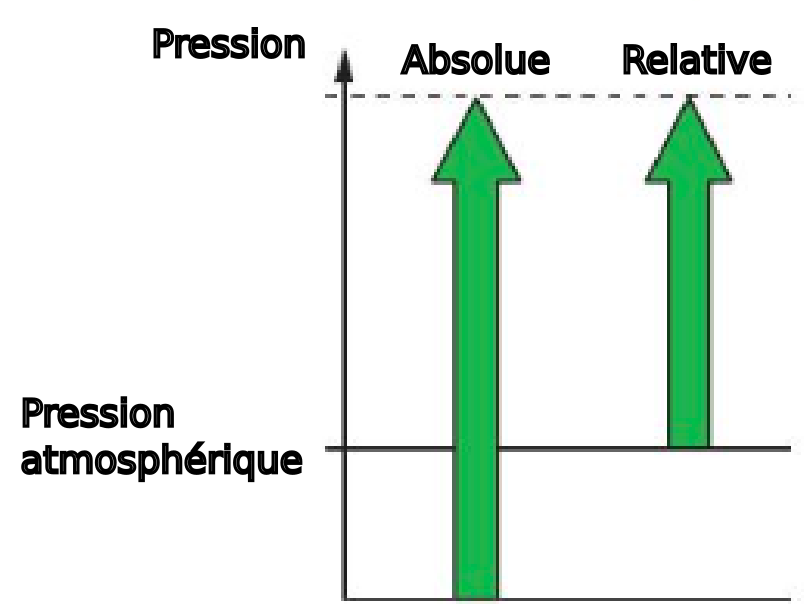
\includegraphics[width=\textwidth]{images/cours1.png}}
\end{minipage}%

\newpage

\fcolorbox{black}{white}{\textbf{\ding{203} Loi de Boyle-Mariotte}}\\
\vspace{-6mm}

\begin{itemize}[label=\textbullet, font=\LARGE \color{black}]
    \item 
\noindent%
\begin{minipage}{.65\textwidth}%
\ctext{A température constante, pour une quantité de gaz donnée, le produit de la pression $p$ par le volume $V$ du gaz est constant : }
\end{minipage}%
\hfill
\begin{minipage}{.23\textwidth}%
\ctext{$$p\times V = constante$$}
\end{minipage}%
\vspace{-6mm}
    \item 
    \noindent%
\begin{minipage}{.90\textwidth}%
\ctext{Le volume occupé par un gaz est inversement proportionnel à la pression de ce gaz. }
\end{minipage}%
\end{itemize}
\vspace{-6mm}
\noindent%
\begin{minipage}{.33\textwidth}%
\fbox{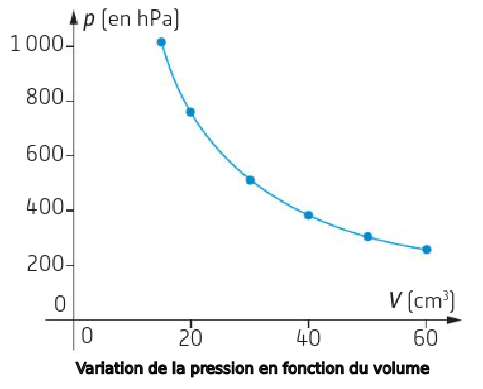
\includegraphics[width=\textwidth]{images/cours2.png}}
\end{minipage}%
\hfill
\begin{minipage}{.33\textwidth}%
\fbox{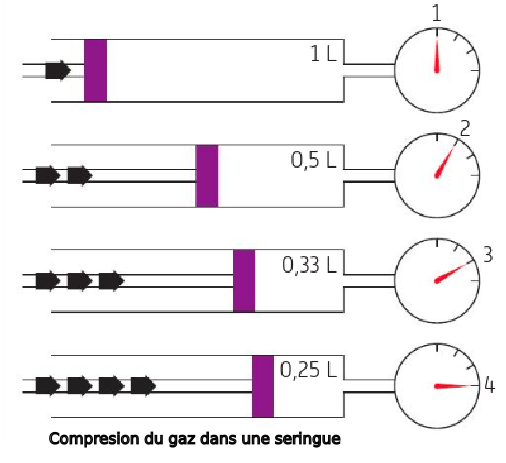
\includegraphics[width=\textwidth]{images/cours3.png}}
\end{minipage}%



\fbox{\textbf{Exercice 1 }} QCM : Parmi les trois propositions, choisissez la bonne réponse. 

    \begin{tabular}{|C{0.5cm} p{5.5cm}|C{3cm}|C{3cm}|C{3cm}|}
         \hline
       \ding{202} &L'unité du système international de la pression est & $\Box $ ~~le bar& $\Box $ ~~l'atmosphère & \Checkedbox   ~~le pascal\\
         \hline
      \ding{203}&Quelle est la relation entre la pression et la force pressante  & $\Box $ ~~$p=F \times S$ & \Checkedbox ~~$F=p \times S$  & $\Box $ ~~ $F=\dfrac{S}{P}$ \\
         \hline
         \ding{204} &Pour une même surface, si la force pressante augmente  que fait la pression &$\Box $ ~~ elle diminue& \Checkedbox ~~ elle augmente & $\Box $ elle reste constante  \\
         \hline
         \ding{205} &Pour une même force pressante que peut on faire pour augmenter une pression & \Checkedbox ~~ diminuer la surface de contact& $\Box $ augmenter la surface de contact& $\Box $ ~~ on ne peut pas la modifier\\
         \hline
         \ding{206}& La pression atmosphérique est environ égale à  &\Checkedbox ~~ $1\times 10^5$~Pa& $\Box $ $1\times 10^{-5} $~Pa& $\Box $ ~~ $1\times 10^5$~Bar \\
         \hline
         \ding{207}&Quel appareil ne permet pas de mesurer la pression & $\Box $ ~~ un baromètre & \Checkedbox ~~  un manomètre & $\Box $ ~~  un anémomètre \\
         \hline
         \ding{208} &Pour une même quantité de gaz, si la pression augmente que fait le volume&\Checkedbox ~~ il diminue& $\Box$ il augmente &$\Box$ ~~ il reste inchangé\\
         \hline
    \end{tabular}

\newpage

\fbox{\textbf{Exercice 2 - compléter le tableau suivant : }}

\begin{center}
    \renewcommand{\arraystretch}{3}
    \begin{tabular}{|p{6cm}|C{2cm}|C{2cm}|C{2cm}|}
         \hline
      Forme à utiliser & $p$ & $F$ & $S$ \\
         \hline 
         Exemple 1 \newline \correction{$F = p \times S$} &  1,013 bar \newline \correction{$= 1{,}013 \times 10^5$~Pa} & \correction{$5{,}065 \times 10^4$~N} & 0,5 $m^2$\\
         \hline
         Exemple 2 \newline \correction{$p = \dfrac{F}{S}$} & \correction{$\approx 7{,}8 \times 10^4$~Pa} & 50 N & 6,4 $cm^2$ \newline \correction{$= 6{,}4\times 10^{-4}$~$m^2$}\\
         \hline 
         Exemple 3 \newline \correction{$S = \dfrac{F}{p}$} & $2 \times 10^5$~Pa & 50 N & \correction{$2{,}5 \times 10^{-4}$~$m^2$}\\
         \hline
    \end{tabular}
\end{center}

\vfill 

\fbox{\textbf{Exercice 3 }}

\vspace{-3mm}

\noindent%
\begin{minipage}{.36\textwidth}%
Un apnéiste inspire à la surface 6 L d'air à la pression atmosphérique. \'A l'aide de la loi de Boyle-Mariotte, calculer en L, le volume occuper par cet air à 20 m de profondeur, sachant que la pression augmente de 1 bar tous les 10 m.  
\end{minipage}%
\hfill
\begin{minipage}{.57\textwidth}%
\correction{
\textbf{Données :}
\begin{itemize}
    \item $p_1 = 1$~bar (à la surface), \quad $V_1 = 6$~L
    \item À 20~m : $p_2 = 1 + 2 \times 1 = 3$~bar
\end{itemize}
\textbf{Application de la loi de Boyle-Mariotte :}
$$p_1 \times V_1 = p_2 \times V_2$$
$$V_2 = \frac{p_1 \times V_1}{p_2} = \frac{1 \times 6}{3} = \mathbf{2~L}$$
Le volume de l'air est divisé par 3 en profondeur.
}
\end{minipage}%

\vfill 

\fbox{\textbf{Exercice 4 }}

Un ballon de baudruche peu gonflé et fermé est posé sous une cloche à vide. 

\begin{enumerate}
    \item Pourquoi ce ballon augmente-t-il de volume quand on chasse l'air sous la cloche à vide ? \\[2mm]
    \correction{Lorsqu'on chasse l'air sous la cloche, la pression extérieure diminue. D'après la loi de Boyle-Mariotte, à température constante, une diminution de pression entraîne une augmentation de volume. La pression intérieure du ballon devenant supérieure à la pression extérieure, le ballon se gonfle.}\\[2mm]

    \item Quelle doit être la pression sous la cloche pour que le ballon triple de volume ? \\[2mm]
    \correction{
    On cherche $p_2$ sachant que $V_2 = 3 \times V_1$ et $p_1 = 1$~bar.
    $$p_1 \times V_1 = p_2 \times V_2 = p_2 \times 3\,V_1$$
    $$p_2 = \frac{p_1}{3} = \frac{1}{3} \approx \mathbf{0{,}33~\text{bar} \approx 3{,}3 \times 10^4~\text{Pa}}$$
    Il faut abaisser la pression sous la cloche à environ $0{,}33$~bar.
    }
\end{enumerate}

\vfill 
\end{fleche}
\end{document}
